\chapter{Podstawy teoretyczne}

\section{Istniejące rozwiązania}
Obecnie w sieci istnieje wiele serwisów umożliwiających porównywanie, ocenianie i tworzenie opinii o produktach. Są to między innymi cokupić.pl,  ceneo.pl, nokaut.pl, skąpiec.pl oraz kupujemy.pl. Wszystkie te serwisy oferują pomoc przy zakupie określonego produktu. Posiadają one aktualną bazę wielu produktów znajdujących się na rynku, przez co umożliwiają użytkownikowi zapoznanie się z nimi. Najbardziej zaawansowanymi projektami, które oferują szereg funkcjonalności są ceneo.pl oraz skąpiec.pl. Oba serwisy umożliwiają przede wszystkim porównywanie cen produktów pochodzących z różnych sklepów. Posiadają one  również rozwinięty system opiniowania produktów. Użytkownicy mogą wypowiadać się na temat każdego produktu, wypisywać jego wady i zalety, a także oceniać, czy opinie innych użytkowników są przydatne. Funkcjonalność udostępniana przez te serwisy została również wdrożona w projekcie RevCommunity. W systemie duży nacisk został położony na stworzenie algorytmu rankingowego, który umożliwia ocenianie recenzji w sposób jak najbardziej wiarygodny. Ten element systemu sprawia, że jest on konkurencyjny w stosunku do wyżej wymienionych portali. 

Serwis cokupić.pl jest nastawiony przede wszystkim na zbieranie recenzji od kupujących na temat produktów. Nie obrazuje on jednak przydatności danej recenzji. Jest tylko przedstawiona informacja ilu użytkowników poleca daną recenzję. To nie wystarcza, by kupujący miał pewność, że opinia nie jest zakłamana. Aplikacje ceneo.pl i skąpiec.pl są głównie ukierunkowane na porównanie cen produktów i dostarczenia informacji o ich dostępności na rynku. Mniejszy nacisk natomiast jest kładziony na kwestie związane z opinią produktu i jej wiarygodnością.  W przypadku serwisów nokaut.pl oraz kupujemy.pl, użytkownik nie ma możliwości oceny przydatność opinii danego produktu. Użytkownik może wystawić ocenę dla produktu oraz napisać opinię na jego temat, jednak jego opinia nie zostanie przez nikogo oceniona. Z tego powodu wiele opinii może być zakłamanych, czego konsekwencją jest wprowadzanie użytkownika w błąd. 

Na rynku zdecydowanie brakuje aplikacji, która udostępniałaby użytkownikom rzetelne informacje na temat produktów oraz opinii o nich. Aplikacja RevCommunity ma zadatki na taką aplikację ze względu na prezentowaną funkcjonalność oraz zaimplementowany algorytm rankingowy do oceny wiarygodności opinii o produktach. 



\section{Grafowa baza danych}

Projekt RevCommunity przyjmuje formę portalu społecznościowego bogatego w powiązania między różnymi jego elementami. Użytkownicy mogą obserwować produkty i subskrybować kanały innych użytkowników. Kategorie produktów mają strukturę drzewiastą. Taka specyfika systemu nasuwa pytanie, czy zastosowanie popularnego relacyjnego modelu danych jest najlepszym rozwiązaniem. W porównaniu do RBD model grafowy bardziej naturalnie reprezentuje rzeczywistość. Dużo łatwiej odwzorować struktury obiektowe na węzły i łuki grafu niż tabele powiązane kluczami obcymi czy dodatkowymi tabelami. Dlatego między obiektowymi językami programowania, a RBD często stosowana jest warstwa ORM, która pełni rolę pośrednika. Duże znaczenie ma tutaj wydajność obu podejść. Grafowe bazy danych okazują się niebywale wydajne przy zapytaniach opierających się na połączeniach między elementami. RBD wręcz przeciwnie, ponieważ każde zapytanie odwołujące się do powiązanych tabel wymaga kosztownego połączenia kilku tabel. Model grafowy rozwiązuje również problem przechowywania struktur drzewiastych.
Odnośnie samej zasady działania grafowych baz danych można powiedzieć, że dane są reprezentowane przez węzły i~łuki. Węzły to instancje obiektów(odpowiedniki rekordów w~RBD). Posiadają atrybuty i~mogą być powiązane z~innymi węzłami. Łuki natomiast reprezentują relacje między wierzchołkami grafu. Każdy łuk musi posiadać węzeł początkowy i~końcowy, oraz etykietę oznaczającą typ relacji. Możliwe jest również definiowanie atrybutów powiązań, czyli tak zwane bogate relacje (rich relationship). Ze względu na kierunek można wyróżnić trzy rodzaje łuków:

\begin{itemize}
\item Wyjściowe
\item Wejściowe
\item Nieskierowane
\end{itemize}

\noindent
Schemat działania grafowej bazy danych reprezentuje rysunek \ref{fig:dbschema}

\begin{figure}[H]
	\centering
	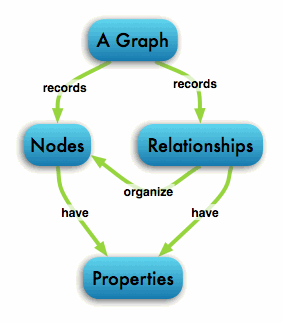
\includegraphics[scale=1]{images/graphdb.png}
	\caption{Schemat działania grafowej bazy danych}
	 \caption*{\small Źródło: \emph{http://assets.neo4j.org/img/propertygraph/graphdb-gve.png}}
	\label{fig:dbschema}
\end{figure}

Do zarządzania zawartością grafowych baz danych stworzono specjalne języki zapytań, pełniące role analogiczne do języka SQL.
Dwa najpopularniejsze języki z tej dziedziny to Gremlin i Cypher. Oba języki umożliwiają budowanie zapytań przechodzenia po grafie, tzn. można zdefiniować pewien schemat połączeń między węzłami i na jego podstawie realizowane będzie wyszukiwanie elementów grafu. Cypher jest znacznie łatwiejszy do zrozumienia i nauki, oraz posiada większe wsparcie w postaci dokumentacji i integracji z np. Neo4j. Istnieją jednak zapytania, których nie da się wykonać za pomocą Cypher. Gremlin daje większe możliwości budowania grafu oraz definiowania sposobu jego przeszukiwania, jednak Cypher, który samodzielnie wyznacza algorytmy wyszukiwania, działa znacznie szybciej w większości przypadków. Składnia języka Cypher nie jest specjalnie skomplikowana i często nawiązuje do języka SQL. Najważniejszym elementem zapytania jest klauzula MATCH, w której zawarty jest kontekst grafowy. Najprostsze polecenie może wyglądać następująco:

\begin{figure}[H]
	\centering
	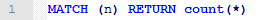
\includegraphics{images/cypher_q1.png}
\end{figure}

W przykładzie zliczono liczbę wszystkich węzłów w grafie. Aby bardziej wykorzystać grafowy charakter bazy danych, możemy zdefiniować schemat połączeń, które nas interesują, a następnie wybrać z dopasowanych wyników interesujące elementy. Zakładając, że w grafie mamy użytkowników, którzy mogą pisać recenzje za pomocą poniższego zapytania, pobierzemy wszystkie napisane recenzje przez użytkownika o loginie jkowalski:

\begin{figure}[H]
	\centering
	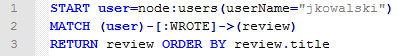
\includegraphics{images/cypher_q2.png}
\end{figure}

Widzimy tutaj nową klauzulę START, która jak nazwa wskazuje, pozwala zdefiniować początkowy węzeł od którego rozpocznie się dopasowanie zawarte w klauzuli MATCH. W zapytaniu użyliśmy dwóch zmiennych - user i review. Do zmiennej user przypisujemy węzeł, który posiada wartości "jkowalski" w polu userName(część indeksu o nazwie "users"). Dalej dla tego wierzchołka wyszukane są wszystkie wyjściowe łuki o etykiecie "WROTE". Dzięki temu udało się dojść do węzłów recenzji, które zwrócono przy pomocy klauzuli RETURN. Ostatnia klauzula definiuje sortowanie po tytule recenzji w sposób analogiczny do języka SQL. Warto tutaj zwrócić uwagę na skalowalność grafowych baz danych w porównaniu do modelu relacyjnego. Gdyby spróbować napisać powyższe zapytanie w języku SQL, musielibyśmy połączyć dwie tabele użytkowników i recenzji. Koszt takiego połączenia jest tym większy im więcej rekordów zawiera każda z tabel. W rzeczywistych systemach z czasem danych przybywa, więc aplikacja działałaby coraz wolniej. Natomiast w grafowej bazie danych węzły nie są zależne od siebie, a dostęp do ich powiązań jest bardzo szybki, dlatego czas wykonania zapytania pozostałby stały mimo rozrastania się grafu. Różnica wydajności między podejściami wzrosłaby, gdyby w zapytaniu dodać kolejne połączenie np. dotyczące komentarzy recenzji. W takim przypadku w RBD konieczne byłoby połączenie trzech tabel, co przy dużej liczbie rekordów byłoby bardzo kosztowne.


\section{Podstawy do stworzenie algorytmu rankingowego}
\label{sec:algTeotia}

Jak wspomniano w rozdziale drugim (NIE MOŻE BYĆ ROZDZIAŁ DRUGI, BO MA KILKA PODROZDZIAŁÓW, WIĘC NALEŻY ZMIENIĆ ALBO NA "jak wspomniano w rozdziale pierwszym" ALBO "W PODROZDZIALE XX ROZDZIAŁU DRUGIEGO"), wiele istniejących systemów opiera się o proste metody oceniania treści, które często okazują się zawodne. Jedną z często spotykanych praktyk jest zastosowanie średniej arytmetycznej do obliczenia ostatecznej oceny widocznej dla użytkowników danego serwisu, a także wykorzystywanej np. do sortowania wyników wyszukiwania czy też porównywania pewnych treści. Przykładem systemu wykorzystującego wspomniany mechanizm jest popularny serwis internetowy cokupić.pl, dający użytkownikom możliwość oceniania produktów. Rozważmy scenariusz, w którym użytkownik korzysta z systemu, w celu znalezienia najlepiej ocenianego przez internautów telefonu komórkowego. Załóżmy, że po zastosowaniu odpowiednich filtrów użytkownikowi przedstawione zostają dwa produkty - A i B. Pierwszy z nich został oceniony przez pięćdziesięciu użytkowników i posiada średnią ocenę 3.5. Drugi oceniły tylko dwie osoby, przydzielając oceny 3 i 5, zatem jego średnia ocena wynosi 4. Średnia ocena produktu B jest nieznacznie wyższa, zatem zostaje on zaprezentowany użytkownikowi jako pierwszy, podczas gdy produkt A posiada znacznie więcej ocen, a~tym samym wiarygodność jego średniej oceny jest wyższa, co może mieć duży wpływ na decyzję użytkownika. Warto zauważyć, że w opisanym podejściu brakuje odniesienia średniej oceny produktu do innych ocen w systemie, przez co porównywanie produktów czy też budowanie właściwego rankingu, jest utrudnione.

Aby uniknąć wspomnianych problemów, zaproponowano podejście oparte na średniej Bayesa. Średnia Bayesa jest metodą obliczania wartości średniej populacji wraz z uwzględnieniem pewnych zewnętrznych danych, związanych z rozważaną populacją. Dodanie czynnika zewnętrznego ma na celu zredukowanie wpływu pojedynczych wartości, odbiegających od średniej, na ostateczny wynik. Dodatkowo czynnik ten pełni rolę wartości domyślnej, czyli takiej, do której dąży wartość średniej w przypadku małego zbioru danych.\cite{bayesWiki} Poniżej przedstawiono wzór średniej Bayesa.

\begin{equation}
\bar{x}=\frac{Cm+nx}{C+n}
\end{equation}
gdzie:\\
C - stała wartość odpowiadająca wielkości typowego zbioru danych\\
m - wartość domyślna\\
x - średnia arytmetyczna zbioru danych\\
n - liczba elementów zbioru\\


Należy zaznaczyć, że dobór wartości domyślnej m i stałej C może zależeć od celu obliczeń, charakterystyki zbioru danych i intuicji osoby wykonującej obliczenia.

\section{Użyte technologie}
Projekt został stworzony przy użyciu technologii webowych, aby umożliwić swobodne korzystanie z~aplikacji z wykorzystaniem przeglądarki internetowej. Do stworzenia projektu zostały użyte:
\begin{itemize}
\item język JavaScript - Skryptowy język programowania. Przy jego pomocy możliwe jest tworzenie dynamicznych stron internetowych.\cite{js}
\item framework ExtJs - Platforma stworzona w języku JavaScript, zawiera szereg funkcjonalności oraz komponentów, które umożliwiają szybką budowę strony internetowej.\cite{extjs}
\item grafowa baza danych Neo4J - Darmowa, zaimplementowana w języku Java baza danych. Struktura bazy oparta jest na grafie.
\item Java EE (ang. \textit{Enterprise Edition}) - Standard tworzenia aplikacji w języku programowania Java, oparty o wielowartwową architekturę komponentową.\cite{javaee}
\item framework Spring - Rozbudowana platforma, stanowi szkielet tworzenia aplikacji w języku Java w standardzie Java EE.\cite{springAction}
\item LESS (ang. \textit{Leaner CSS}) - Aplikacja rozszerzająca możliwości CSS (ang. \textit{Cascading Style Sheets}).\cite{LESS}
\item HTML (ang. \textit{HyperText Markup Language}) - Hipertekstowy język znaczników, szeroko wykorzystywany do tworzenia stron internetowych. Pozwala opisać strukturę informacji zawartych wewnątrz strony internetowej poprzez odpowiednie ich formatowanie.\cite{html}
\item wzorzec REST (ang. \textit{Representational State Transfer}) - Wzorzec architektury oprogramowania wykorzystujący protokół HTTP, wprowadzający dobre praktyki dotyczące tworzenia aplikacji wielowarstwowych.\cite{restWww}
\end{itemize}
